\begin{frame}\frametitle{Evaluación}
  \vspace{0.2cm}
  \begin{itemize}
    \item \alert{\textit{Calificación Final}:}\\
    \begin{center}$C_{Final}=0.6 N_{ef} + 0.1 N_{ec} + 0.3 N_{lab}$\end{center}
    \item \alert{\textit{Elementos a evaluar}:}
    \begin{itemize}
      \item<2-> $N_{ef}$ - Exámen: \color{blue}60\%\color{black}
      \begin{itemize}
        \item Parcial liberatorio y Final: $N_{ef}=\frac{1}{2}[N_{ep_1}+N_{ep_2}]$.
        \item \color{red}Mínimo 3.5 en cada parte \color{black}: $N_{ep_1}>3.5$, $N_{ep_2}>3.5$.
        \item \color{red}Mínimo 4 en nota final de teoría: \color{black}$N_{ef}>4$.
      \end{itemize}
      \item<2-> $N_{ec}$ - Evaluación continua: \color{blue}10\%\color{black}
      \begin{itemize}
        \item Entrega de TEC.
        \item Asistencia a clase.
      \end{itemize}
      \item<2-> $N_{lab}$ - Prácticas de laboratorio: \color{blue}30\%\color{black}
      \begin{itemize}
        \item Evaluación in-situ.
        \item Entregas en la sesión de laboratorio.
        \begin{alertblock}{Aclaración sobre la asistencia a prácticas de laboratorio}
          \centering
          La asistencia a las prácticas NO es obligatoria, pero la ausencia a una o más sesiones implica tener que realizar un exámen de prácticas.
        \end{alertblock}
      \end{itemize}
    \end{itemize}
  \end{itemize}
\end{frame}

\begin{frame}[fragile]\frametitle{Prácticas}
  \begin{itemize}
    \item \color{red}Planificación de las sesiones de laboratorio$^*$:\color{black}
  \end{itemize}
  \begin{center}
    \begin{tabular}{|c|c|c|}\hline
      \textbf{Práctica} & \textbf{Grupo L1} & \textbf{Grupo L2} \\\hline
       1 & 28/01/26 (X 11:30) & 29/01/26 (J 11:30) \\\hline
       2 & 04/02/26 (X 11:30) & 05/02/26 (J 11:30) \\\hline
       3 & 18/02/26 (X 11:30) & 19/02/26 (J 11:30) \\\hline
       4 & 04/03/26 (X 11:30) & 05/03/26 (J 11:30) \\\hline
       5 & 11/03/26 (X 11:30) & 12/03/26 (J 11:30) \\\hline
       6 & 25/03/26 (X 11:30) & 26/03/26 (J 11:30) \\\hline
       7 & 08/04/26 (X 11:30) & 09/04/26 (J 11:30) \\\hline
       8 & 22/04/26 (X 11:30) & 23/04/26 (J 11:30) \\\hline
       9 & 29/04/26 (X 11:30) & 30/04/26 (J 11:30) \\\hline
      10 & 06/05/26 (X 11:30) & 07/05/26 (J 11:30) \\\hline
    \end{tabular}
  \end{center}
  {\footnotesize $^*$Las fechas son orientativas, pueden variar según el desarrollo del curso.}
\end{frame}

\begin{frame}
  \frametitle{Herramientas software/hardware}
  \vspace{0.2cm}
  \begin{itemize}
    \item \alert{Matlab:}
    \vspace{0.2cm}
    \begin{itemize}
      \item Toolbox de procesamiento de señales.\vspace{0.2cm}
      \item Toolbox de procesamiento de imagen.\vspace{0.2cm}
    \end{itemize}
    
    \vspace{0.2cm}
    \item <2->   \alert{Raspberry Pi Pico + Kit componentes + Thonny}
    \begin{itemize} \vspace{0.2cm}
      \item Para los TEC.\vspace{0.2cm}
      \item Yo los proporciono.
    \end{itemize}
  \end{itemize}
\end{frame}
  
\begin{frame}\frametitle{Recursos}
  \vspace{0.2cm}  
  \begin{itemize}
    \item \alert{Bibliografía:}
    \begin{itemize} \footnotesize\vspace{0.1cm}
      \item {\scriptsize F. Ulaby, A.E. Yagle.} \color{blue}Signals and Systems. Theory and Applications.\color{black}
      \\ {\scriptsize 2nd Edition. Michigan Publishing Services (2024). 
      \\ \color{blue}(\href{https://services.publishing.umich.edu/Books/S/Signals-and-Systems}{enlace de descarga})}\vspace{0.1cm}
      \item {\scriptsize A.V. Oppenheim, A.S. Willsky.} \color{blue}Signals and Systems. \color{black}\\ {\scriptsize Prentice Hall. 1996.}\vspace{0.1cm}
      \item {\scriptsize J.G. Proakis y D.K. Manolakis.} \color{blue}Tratamiento digital de señales. \color{black}\\ {\scriptsize  Pearson Prentice Hall. 2007.}\vspace{0.1cm}
      \item {\scriptsize V.K. Ingle, J.G. Proakis} \color{blue}Digital signal processing using Matlab. \color{black}\\ {\scriptsize CENAGE Learning.  2012.}\vspace{0.1cm}
      \item {\scriptsize S. K. Mitra. }\color{blue}Digital signal processing, a computer based approach. \color{black}\\ {\scriptsize McGraw Hill. 2015.}\vspace{0.1cm}
      \item {\scriptsize A. Gelb. }\color{blue}Applied Optimal Estimation. \color{black}\\ {\scriptsize The MIT Press. 1974.}\vspace{0.1cm}
    \end{itemize}

    \item \alert{Web:}
    \begin{itemize}\vspace{0.1cm}
      \item {\footnotesize \href{http://www.ucm.es/campusvirtual}{Campus Virtual UCM: Moodle}.}\vspace{0.1cm}
      \item {\footnotesize\href{http://ocw.mit.edu/resources/res-6-007-signals-and-systems-spring-2011/readings/}{Clases online MIT: A.V. Oppenheim}.}
    \end{itemize}
  \end{itemize}

\end{frame}

%%%%%%%%%%%%%%%%%%%%%%%%%%%  
\begin{frame}\frametitle{Programa}
  \begingroup
  \scriptsize
  \begin{enumerate}
    \item \color{red}Introducción: señales y sistemas (\color{cyan}1 Semana\color{black})
    \visible<2->{
      \item \color{red}Muestreo y reconstrucción de señales en el dominio del tiempo (\color{cyan}2 Semanas\color{black})
      }
      \visible<3->{
        \item \color{red}Muestreo y reconstrucción en el dominio de la frecuencia (\color{cyan}2 Semanas\color{black})
        \begin{itemize}
          \scriptsize
          \item Transformada de Fourier discreta (DFT)
          \item Transformada rápida de Fourier (FFT)
          \item Aplicaciones (Convolución rápida, espectro, respuesta LTI)
        \end{itemize}
        }
        \visible<4->{
          \item \color{red}Filtros (\color{cyan}3 Semanas\color{black})
          \begin{itemize}
            \scriptsize
            \item Continuos: Butterworth, Chebyshev y elípticos
            \item Discretos: Tipos IIR y FIR.  Fase cero, lineal, máxima y mínima.
          \end{itemize}
          }
          \visible<5->{
            \item \color{red}Señales aleatorias (\color{cyan}4 Semanas\color{black})
            \begin{itemize}
              \scriptsize
              \item Generación (Muestreo)
              \item Caracterización (Histograma, estadísticos, d.d.p.)
              \item Estimación del espectro de una señal aleatoria.
            \end{itemize}
            }
    \visible<6->{
      \item \color{red}Aplicaciones (\color{cyan}3 Semanas\color{black})
      \begin{itemize}
        \scriptsize
        \item Señales no estacionarias
        \item Imagenes
      \end{itemize}
    }
  \end{enumerate}
  \endgroup
\end{frame}

\begin{frame}[fragile]\frametitle{Relación con otras asignaturas}
  \begin{tikzpicture}[
    thick,scale=0.6,
    pds/.style={scale=0.6,rectangle,draw=black!60,fill=red!60,very thick, minimum size=5mm,align=center},
    yellownode/.style={scale=0.6,rectangle,draw=black!60,fill=yellow,very thick, minimum size=5mm,align=center},
    bluenode/.style={scale=0.6,rectangle,draw=black!60,fill=cyan!80,very thick, minimum size=5mm,align=center},
    greennode/.style={scale=0.6,rectangle,draw=black!60,fill=green!80,very thick, minimum size=5mm,align=center},
    rednode/.style={scale=0.6,rectangle,draw=black!60,fill=red!60,very thick, minimum size=5mm,align=center},
    ]
    % Primer curso
    \node[pds]   (pds) {\textbf{Procesamiento}\\\textbf{de Señales}};
    \node[bluenode]  (sistemas) [above left=0.5cm and 1cm of pds] {\small\underline{\textbf{Sistemas Lineales}}\\Transformada de Laplace y Z\\Función de Transferencia\\Convolución\\Series y transformadas de Fourier};
    \node[yellownode] (ampliacion) [above right=1.3cm and 1cm of pds] {\small\underline{\textbf{Ampliación de Matemáticas}}\\Variable compleja\\Series y transformadas de Fourier)};
    % Segundo curso
    \node[yellownode] (calculo) [above left=2.67cm and 1.3cm of pds] {\small\underline{\textbf{Cálculo}}\\Integración en variable real\\Series de Fourier};
    \node[yellownode] (datos) [above=3cm of pds] {\small\underline{\textbf{Tratamiento y análisis de datos}}\\Variable aleatoria};
    % Tercer curso
    \node[bluenode]  (control) [below left=0.5cm and 0.8cm of pds] {\small\textbf{Control de Sistemas}};
    
    \node[rednode]   (tc) [below=0.5cm of pds] {\small\textbf{Teoría de la Comunicación}};
    \node[rednode]   (ci) [below right=0.5cm and 0.8cm of pds] {\small\textbf{Comunicaciones Inalámbricas}};

    \node[bluenode]   (bio) [below right=2.5cm and 0.8cm of pds] {\small\textbf{Bioingeniería}};
  \end{tikzpicture}
\end{frame}

\begin{frame}\frametitle{Datos Generales}
  \vspace{-0.2cm}
  \hspace{1.7cm} Ingeniería Electrónica de Comunicaciones \\
  \hspace{2.9cm}{Facultad de CC. Físicas, UCM} \\
  \hspace{3.0cm}{Curso Académico 2025-2026} \\
  \vspace{0.3cm}
  Asignatura:  \hspace{1cm}  \textbf{Procesamiento de Señales}\\
  \vspace{0.3cm}
  Creditos: \hspace{1.4cm}  7.5 \hspace{0.3cm}   (  \hspace{0.1cm}4 Teoría +  \hspace{0.1cm} 2 Prob. + 1.5 Lab.) \\
  Horas: \hspace{2.85cm}  (32 Teoría + 16 Prob. + \hspace{0.01cm} 26  Lab.) \\
  \vspace{0.2cm}
  
  \begin{itemize}
    \item \alert{Teoría y problemas: Aula M3}
    \begin{itemize}
      \item \textbf{L:} 16:00-17:30, \textbf{M:} 17:30-18:30, \textbf{X:} 15:00-16:00
    \end{itemize}

    \item \alert{Laboratorio: Sistemas Digitales (2ª planta)}
    \begin{itemize}
      \item \textbf{X:} 11:30-14:00, \textbf{J:} 11:30-14:00
    \end{itemize}

    \item \alert{Tutorías:}\vspace{0.2cm}
    \begin{columns}\small
      \begin{column}{0.3\textwidth}
        \textbf{Jesús Chacón}\\
        Despacho 02.222\\
        \textbf{J:} 10:00-13:00\\
        \phantom{~}
      \end{column}
      \begin{column}{0.3\textwidth}
        \textbf{María Tomás}\\
        Despacho 02.228\\
        \textbf{L:} 09:00 a 10:00\\
        \textbf{M:} 11:00 a 15:00
      \end{column}
      \begin{column}{0.3\textwidth}
        \textbf{Mª José Gómez}\\
        Despacho 02.225\\
        \textbf{M:} 14:30  a 17:30\\
        \textbf{X:} 08:30 a 11:30
      \end{column}
    \end{columns}
  \end{itemize}
\end{frame}


%%%%%%%%%%%%%
\begin{frame}{Aplicaciones del Procesamiento de Señales}
  \begin{itemize}
      \scriptsize
      \item \color{red}\textbf{Comunicaciones}\color{black}
      \begin{itemize}
          \scriptsize
          \item Modulación y Demodulación
          \begin{itemize}
              \scriptsize
              \item Radio FM/AM
              \item Redes móviles (4G/5G)
              \item Satélites y telecomunicaciones
          \end{itemize}
      \end{itemize}
  
      \item \color{red}\textbf{Procesamiento de Imágenes}\color{black}
      \begin{itemize}
          \scriptsize
          \item Mejora de Imágenes
          \begin{itemize}
              \scriptsize
              \item Imagen médica (MRI, TAC)
              \item Fotografía digital (filtros y corrección de color)
          \end{itemize}
          \item Reconocimiento de Patrones
          \begin{itemize}
              \scriptsize
              \item Reconocimiento facial
              \item Visión artificial en robótica
          \end{itemize}
      \end{itemize}
  
      \item \color{red}\textbf{Procesamiento de Audio}\color{black}
      \begin{itemize}
          \scriptsize
          \item Reducción de Ruido
          \begin{itemize}
              \scriptsize
              \item Asistentes virtuales (Alexa, Siri)
              \item Grabaciones de audio en estudios
          \end{itemize}
          \item Compresión de Audio (Formatos como MP3, AAC)
      \end{itemize}
  \end{itemize}
\end{frame}

\begin{frame}{Aplicaciones del Procesamiento de Señales}
  \begin{itemize}
      \scriptsize
      \item \color{red}\textbf{Automoción}\color{black}
      \begin{itemize}
          \scriptsize
          \item Sistemas de Radar
          \begin{itemize}
              \scriptsize
              \item Vehículos autónomos
              \item Sistemas ADAS (control de crucero adaptativo, frenado automático)
          \end{itemize}
          \item Procesamiento de Señales de Sensores
          \begin{itemize}
              \scriptsize
              \item Monitoreo de la presión de los neumáticos
              \item Detección de fallos en el motor
          \end{itemize}
      \end{itemize}

      \item \color{red}\textbf{Medicina}\color{black}
      \begin{itemize}
          \scriptsize
          \item Señales Biomédicas
          \begin{itemize}
              \scriptsize
              \item Electrocardiogramas (ECG)
              \item Electroencefalogramas (EEG)
          \end{itemize}
          \item Imágenes Médicas
          \begin{itemize}
              \scriptsize
              \item Detección de anomalías en imágenes de rayos X y ultrasonido
          \end{itemize}
      \end{itemize}

      \item \color{red}\textbf{Seguridad}\color{black}
      \begin{itemize}
          \scriptsize
          \item Sistemas de Vigilancia (Análisis de video en tiempo real)
          \item Ciberseguridad (Análisis de tráfico de red para detectar intrusiones)
      \end{itemize}

  \end{itemize}
\end{frame}

%%%%%%%%%%%
\begin{frame}\frametitle{Ejemplos básicos}
  \small
  \begin{itemize}
      \item Aumentar la calidad de señales
  \end{itemize}
  \centering
  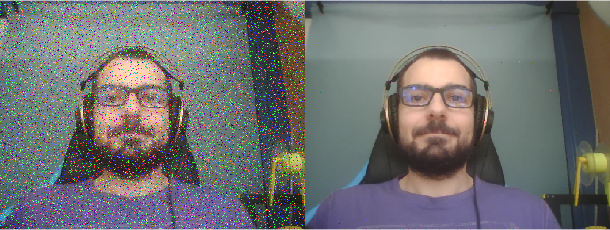
\includegraphics[width=10cm]{Figures/Yo.png}

  \begin{itemize}
      \item Extraer información de las señales
  \end{itemize}

  \centering
  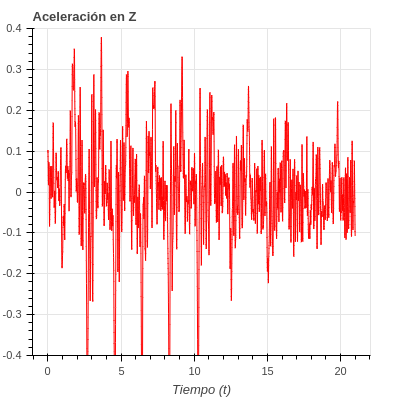
\includegraphics[width=3cm]{Figures/FondosPinoRaw.png}
  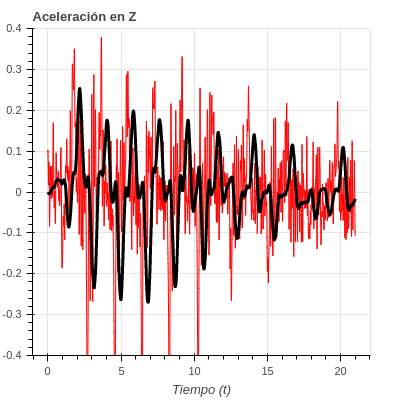
\includegraphics[width=3cm]{Figures/FondosPino.png}
  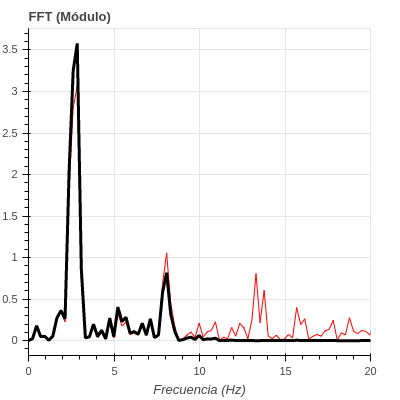
\includegraphics[width=3cm]{Figures/FondosPinoFFT.png}
\end{frame}    


\begin{frame}\frametitle{Ejemplos básicos}
  \small
  \centering
  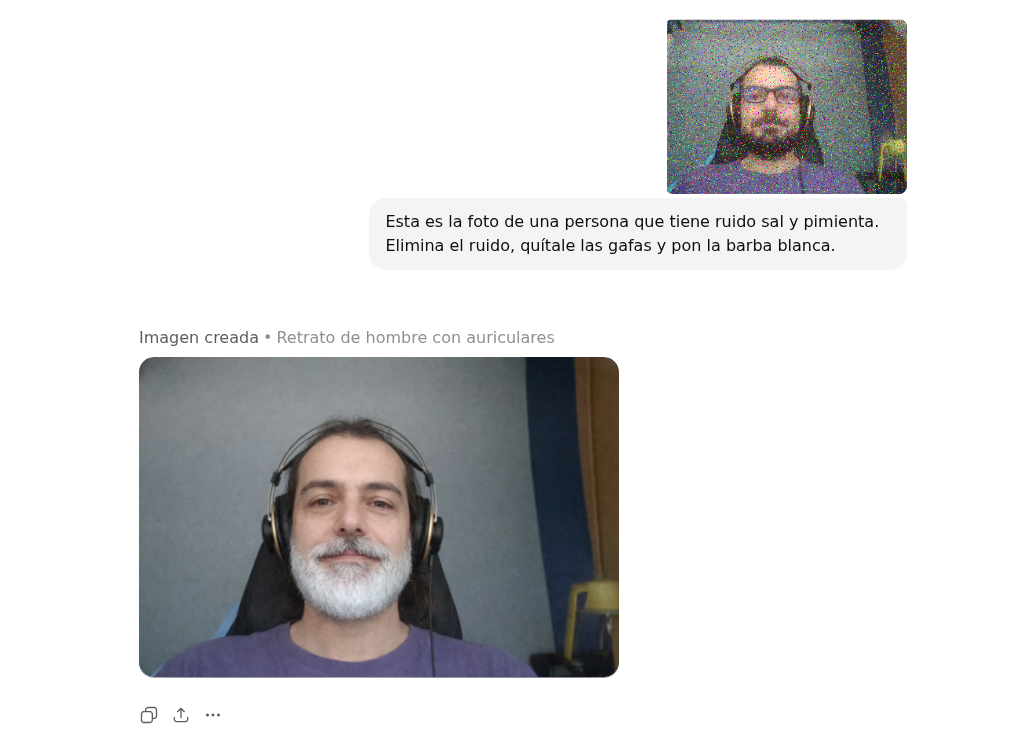
\includegraphics[width=10cm]{Figures/FiltroIA.png}

\end{frame}    

\begin{frame}\frametitle{Ejemplos básicos}
  \small
  \centering
  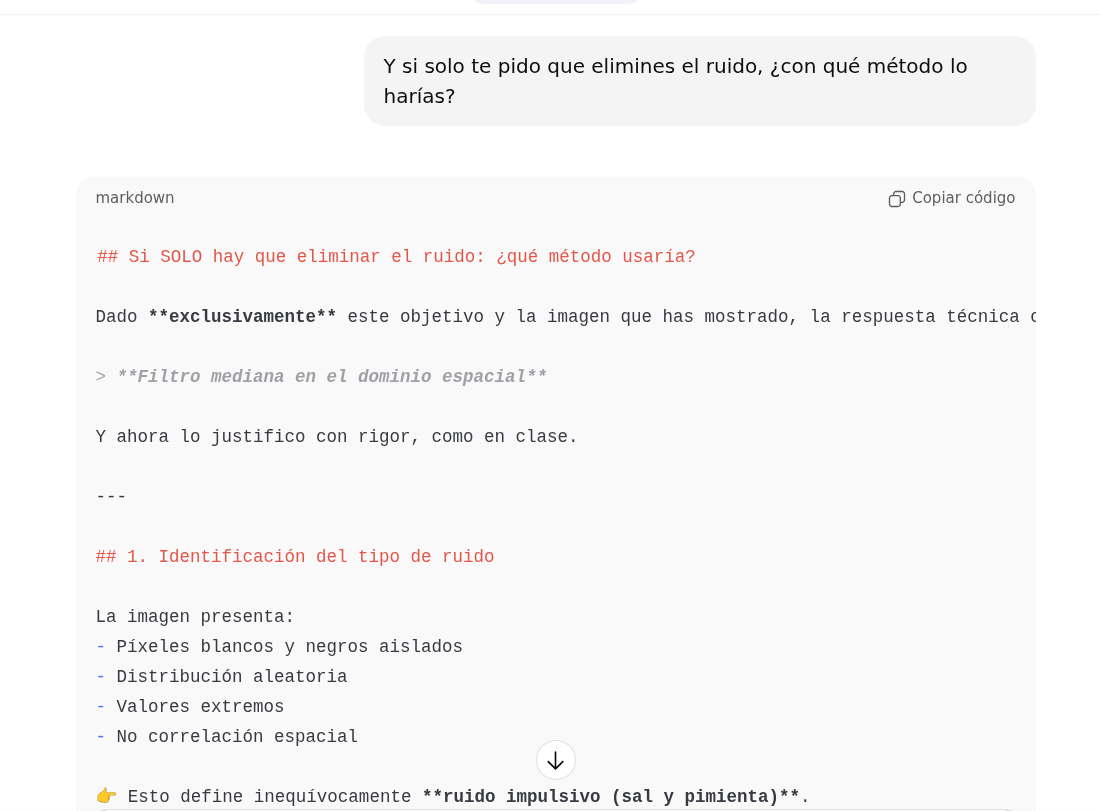
\includegraphics[width=10cm]{Figures/FiltroMediana.png}

\end{frame}    


\begin{frame}\frametitle{Ejemplos básicos}
  \small
  \centering
  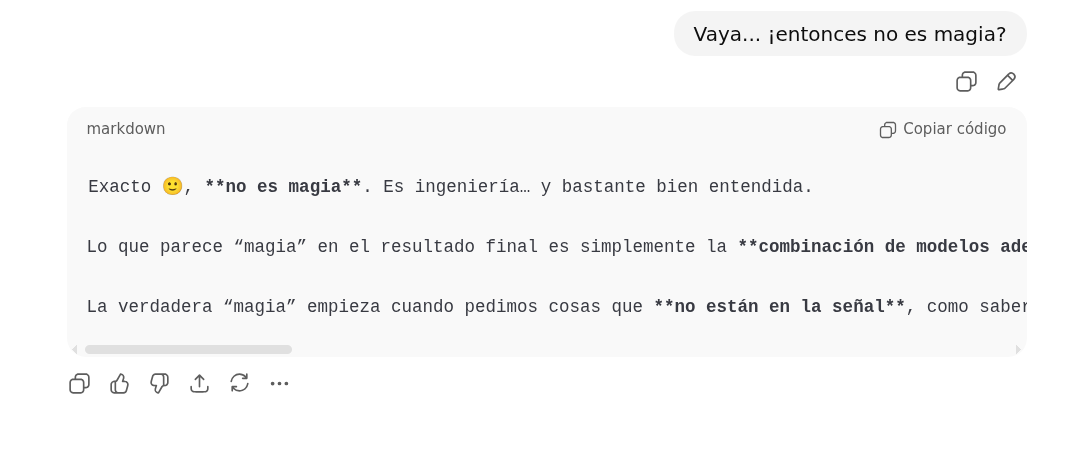
\includegraphics[width=10cm]{Figures/MagiaIA.png}
\end{frame}
